\section{Solution of the incompressible Navier-Stokes equations}\label{sec:ins}

\subsection{Spatial Discretization}\label{sec:ns_space}

To discretize the Navier-Stokes equations~\eqref{eq:ins-momentum} and~\eqref{eq:ins-incomp}, we use a
marker-and-cell (MAC) grid~\cite{Welch:1965jv}: for grid cell center $\x_i$, scalar-valued function $s(\x)$ is
discretized at $\x_i$, and component $\e_a\cdot\vec{v}$ of vector-valued function $\vec{v}(\x)$ at
$\x_i-\sfrac12h\e_a$, where $\e_a$ is a canonical basis vector. Define the centered difference operator
\begin{equation}
    D_a\phi(\x) = \frac{\phi(\x+\sfrac12 h\e_a) - \phi(\x-\sfrac12 h\e_a)}{h},
\end{equation}
for which, \latin{e.g.}, $D_1$ approximates differentiation in the $x$ direction. The discrete divergence,
gradient, and Laplacian operators use centered differences, resulting in a 2-point stencil for each discrete first
derivative and the standard 7-point discrete Laplacian. We also define the centered average operator
\begin{equation}
    A_a\phi(\x) = \frac{\phi(\x+\sfrac12 h\e_a) + \phi(\x-\sfrac12 h\e_a)}2.
\end{equation}
By averaging $u$ in the $y$ direction and $v$ in the $x$ direction, we obtain collocated approximations to $u$ and
$v$ at the center of a cell edge. Averaging, e.g., $u$ in the $x$ direction yields an approximation to $u$ at the
cell center. We can therefore discretize the components of the advection term $\div(\u\otimes\u)$ by
\begin{equation}\label{eq:advection}
    \div[h](\u\otimes\u) :=
    \begin{bmatrix}
        D_1[(A_1 u) (A_1 u)] + D_2[(A_1 v) (A_2 u)] + D_3[(A_1 w) (A_3 u)] \\
        D_1[(A_2 u) (A_1 v)] + D_2[(A_2 v) (A_2 v)] + D_3[(A_2 w) (A_3 v)] \\
        D_1[(A_3 u) (A_1 w)] + D_2[(A_3 v) (A_2 w)] + D_3[(A_3 w) (A_3 w)]
    \end{bmatrix}.
\end{equation}
The symbol $\div[h]$ represents the discrete divergence operator.  \Cref{fig:discretization} illustrates the steps
in computing $D_2[(A_1 v)(A_2 u)]$, which appears in the first component in~\eqref{eq:advection}. Morinishi
\latin{et al.}~\cite{Morinishi:1998us} show that this scheme, $Div. - S2$ in their parlance, is conservative under
the assumption that $\u$ is discretely divergence-free.

\begin{figure}[htb]
    \centering
    \begin{subfigure}{0.33\textwidth}
        \centering
    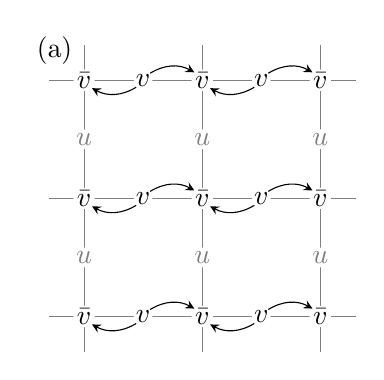
\begin{tikzpicture}[scale=1.5]
        \draw[help lines] (-0.3, -0.3) grid (2.3, 2.3);

        \foreach \x in {0,...,2}
            \foreach \y in {0,...,1}
            {
                \node[circle, inner sep=0pt, color=black!50, fill=white] at (\x, \y+0.5) {$u$};
            }
        \foreach \y in {0,...,2}
        {
            \foreach \x in {0,...,2}
                \node[circle, inner sep=0pt, fill=white] (av\x\y) at (\x, \y) {$\bar{v}$};
            \foreach \x in {0,...,1}
                \node[circle, inner sep=0pt, fill=white] (v\x\y) at (\x+0.5, \y) {$v$};
        }
        \path[-stealth] (v00.south west) edge[bend left] node[midway, below, yshift=+1pt] {} (av00.south east);
        \path[-stealth] (v10.south west) edge[bend left] node[midway, below, yshift=+1pt] {} (av10.south east);
        %\path[-stealth] (v20.south west) edge[bend left] node[midway, below, yshift=+1pt] {} (av20.south east);
        \path[-stealth] (v01.south west) edge[bend left] node[midway, below, yshift=+1pt] {} (av01.south east);
        \path[-stealth] (v11.south west) edge[bend left] node[midway, below, yshift=+1pt] {} (av11.south east);
        %\path[-stealth] (v21.south west) edge[bend left] node[midway, below, yshift=+1pt] {} (av21.south east);
        \path[-stealth] (v02.south west) edge[bend left] node[midway, below, yshift=+1pt] {} (av02.south east);
        \path[-stealth] (v12.south west) edge[bend left] node[midway, below, yshift=+1pt] {} (av12.south east);
        %\path[-stealth] (v22.south west) edge[bend left] node[midway, below, yshift=+1pt] {} (av22.south east);
        %\path[-stealth] (v03.south west) edge[bend left] node[midway, below, yshift=+1pt] {} (av03.south east);
        %\path[-stealth] (v13.south west) edge[bend left] node[midway, below, yshift=+1pt] {} (av13.south east);
        %\path[-stealth] (v23.south west) edge[bend left] node[midway, below, yshift=+1pt] {} (av23.south east);

        \path[-stealth] (v00.north east) edge[bend left] node[midway, below, yshift=+1pt] {} (av10.north west);
        \path[-stealth] (v10.north east) edge[bend left] node[midway, below, yshift=+1pt] {} (av20.north west);
        %\path[-stealth] (v20.north east) edge[bend left] node[midway, below, yshift=+1pt] {} (av30.north west);
        \path[-stealth] (v01.north east) edge[bend left] node[midway, below, yshift=+1pt] {} (av11.north west);
        \path[-stealth] (v11.north east) edge[bend left] node[midway, below, yshift=+1pt] {} (av21.north west);
        %\path[-stealth] (v21.north east) edge[bend left] node[midway, below, yshift=+1pt] {} (av31.north west);
        \path[-stealth] (v02.north east) edge[bend left] node[midway, below, yshift=+1pt] {} (av12.north west);
        \path[-stealth] (v12.north east) edge[bend left] node[midway, below, yshift=+1pt] {} (av22.north west);
        %\path[-stealth] (v22.north east) edge[bend left] node[midway, below, yshift=+1pt] {} (av32.north west);
        %\path[-stealth] (v03.north east) edge[bend left] node[midway, below, yshift=+1pt] {} (av13.north west);
        %\path[-stealth] (v13.north east) edge[bend left] node[midway, below, yshift=+1pt] {} (av23.north west);
        %\path[-stealth] (v23.north east) edge[bend left] node[midway, below, yshift=+1pt] {} (av33.north west);

        \node[black] at (-0.25, 2.25) {(a)};
    \end{tikzpicture}
    \label{fig:adv-x-ave}
    \end{subfigure}%
    \begin{subfigure}{0.33\textwidth}
        \centering
    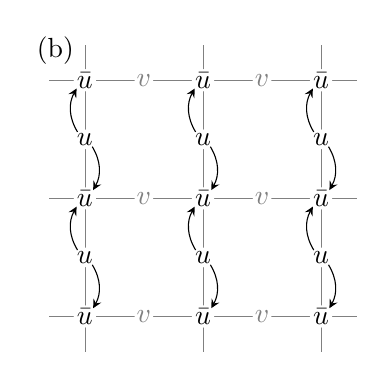
\begin{tikzpicture}[scale=1.5]
        \draw[help lines] (-0.3, -0.3) grid (2.3, 2.3);

        \foreach \x in {0,...,2}
        {
            \foreach \y in {0,...,1}
            {
                \node[circle, inner sep=0pt, fill=white] (u\x\y) at (\x, \y+0.5) {$u$};
            }
            \foreach \y in {0,...,2}
            {
                \node[circle, inner sep=0pt, fill=white] (au\x\y) at (\x, \y) {$\bar{u}$};
            }
        }
        \foreach \x in {0,...,1}
            \foreach \y in {0,...,2}
            {
                \node[circle, inner sep=0pt, color=black!50, fill=white] at (\x+0.5, \y) {$v$};
            }

        \path[-stealth] (u00.south east) edge[bend left] node[midway, below, yshift=+1pt] {} (au00.north east);
        \path[-stealth] (u10.south east) edge[bend left] node[midway, below, yshift=+1pt] {} (au10.north east);
        \path[-stealth] (u20.south east) edge[bend left] node[midway, below, yshift=+1pt] {} (au20.north east);
        %\path[-stealth] (u30.south east) edge[bend left] node[midway, below, yshift=+1pt] {} (au30.north east);
        \path[-stealth] (u01.south east) edge[bend left] node[midway, below, yshift=+1pt] {} (au01.north east);
        \path[-stealth] (u11.south east) edge[bend left] node[midway, below, yshift=+1pt] {} (au11.north east);
        \path[-stealth] (u21.south east) edge[bend left] node[midway, below, yshift=+1pt] {} (au21.north east);
        %\path[-stealth] (u31.south east) edge[bend left] node[midway, below, yshift=+1pt] {} (au31.north east);
        %\path[-stealth] (u02.south east) edge[bend left] node[midway, below, yshift=+1pt] {} (au02.north east);
        %\path[-stealth] (u12.south east) edge[bend left] node[midway, below, yshift=+1pt] {} (au12.north east);
        %\path[-stealth] (u22.south east) edge[bend left] node[midway, below, yshift=+1pt] {} (au22.north east);
        %\path[-stealth] (u32.south east) edge[bend left] node[midway, below, yshift=+1pt] {} (au32.north east);

        \path[-stealth] (u00.north west) edge[bend left] node[midway, below, yshift=+1pt] {} (au01.south west);
        \path[-stealth] (u10.north west) edge[bend left] node[midway, below, yshift=+1pt] {} (au11.south west);
        \path[-stealth] (u20.north west) edge[bend left] node[midway, below, yshift=+1pt] {} (au21.south west);
        %\path[-stealth] (u30.north west) edge[bend left] node[midway, below, yshift=+1pt] {} (au31.south west);
        \path[-stealth] (u01.north west) edge[bend left] node[midway, below, yshift=+1pt] {} (au02.south west);
        \path[-stealth] (u11.north west) edge[bend left] node[midway, below, yshift=+1pt] {} (au12.south west);
        \path[-stealth] (u21.north west) edge[bend left] node[midway, below, yshift=+1pt] {} (au22.south west);
        %\path[-stealth] (u31.north west) edge[bend left] node[midway, below, yshift=+1pt] {} (au32.south west);
        %\path[-stealth] (u02.north west) edge[bend left] node[midway, below, yshift=+1pt] {} (au03.south west);
        %\path[-stealth] (u12.north west) edge[bend left] node[midway, below, yshift=+1pt] {} (au13.south west);
        %\path[-stealth] (u22.north west) edge[bend left] node[midway, below, yshift=+1pt] {} (au23.south west);
        %\path[-stealth] (u32.north west) edge[bend left] node[midway, below, yshift=+1pt] {} (au33.south west);
        \node[black] at (-0.25, 2.25) {(b)};
    \end{tikzpicture}
    \label{fig:adv-y-ave}
    \end{subfigure}%
    \begin{subfigure}{0.33\textwidth}
        \centering
    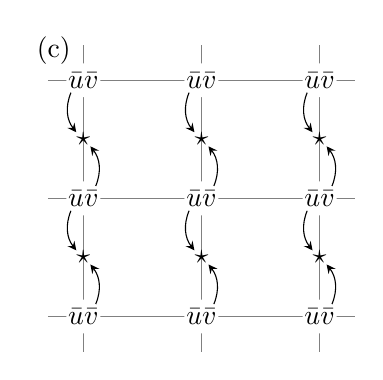
\begin{tikzpicture}[scale=1.5]
        \draw[help lines] (-0.3, -0.3) grid (2.3, 2.3);

        \foreach \x in {0,...,2}
            \foreach \y in {0,...,2}
                \node[circle, inner sep=0pt, fill=white] (uv\x\y) at (\x, \y) {$\bar{u}\bar{v}$};
        \foreach \x in {0,...,2}
            \foreach \y in {0,...,1}
                \node[circle, inner sep=0pt] (duv\x\y) at (\x, \y+0.5) {$\star$};

        \path[stealth-] (duv00.south east) edge[bend left] (uv00.north east);
        \path[stealth-] (duv10.south east) edge[bend left] (uv10.north east);
        \path[stealth-] (duv20.south east) edge[bend left] (uv20.north east);
        %\path[stealth-] (duv30.south east) edge[bend left] (uv30.north east);
        \path[stealth-] (duv01.south east) edge[bend left] (uv01.north east);
        \path[stealth-] (duv11.south east) edge[bend left] (uv11.north east);
        \path[stealth-] (duv21.south east) edge[bend left] (uv21.north east);
        %\path[stealth-] (duv31.south east) edge[bend left] (uv31.north east);
        %\path[stealth-] (duv02.south east) edge[bend left] (uv02.north east);
        %\path[stealth-] (duv12.south east) edge[bend left] (uv12.north east);
        %\path[stealth-] (duv22.south east) edge[bend left] (uv22.north east);
        %\path[stealth-] (duv32.south east) edge[bend left] (uv32.north east);
                                                                           
        \path[stealth-] (duv00.north west) edge[bend left] (uv01.south west);
        \path[stealth-] (duv10.north west) edge[bend left] (uv11.south west);
        \path[stealth-] (duv20.north west) edge[bend left] (uv21.south west);
        %\path[stealth-] (duv30.north west) edge[bend left] (uv31.south west);
        \path[stealth-] (duv01.north west) edge[bend left] (uv02.south west);
        \path[stealth-] (duv11.north west) edge[bend left] (uv12.south west);
        \path[stealth-] (duv21.north west) edge[bend left] (uv22.south west);
        %\path[stealth-] (duv31.north west) edge[bend left] (uv32.south west);
        %\path[stealth-] (duv02.north west) edge[bend left] (uv03.south west);
        %\path[stealth-] (duv12.north west) edge[bend left] (uv13.south west);
        %\path[stealth-] (duv22.north west) edge[bend left] (uv23.south west);
        %\path[stealth-] (duv32.north west) edge[bend left] (uv33.south west);
        \node[black] at (-0.25, 2.25) {(c)};
    \end{tikzpicture}
    \label{fig:adv-y-diff}
    \end{subfigure}%
    \caption{%
        A cross-section illustrating the steps in computing the $D_2[(A_2 u) (A_1 v)]$
        term of the first component of the advection. The horizontal and vertical
        velocity component discretization locations are marked by $u$ and $v$,
        respectively. Arrows emanate from a point contributing to a stencil and point to
        the center of the stencil.
        (a) $A_1$ averages $v$ in the $x$ direction, yielding an approximation $\bar{v}$
        at grid vertices (in 3D, centers of cell edges for which $x$ and $y$ are
        constant).
        (b) $A_2$ averages $u$ in the $y$ direction, yielding an approximation $\bar{u}$
        at the same points as (a). The quantities $A_1 v$ and $A_2 u$ are collocated and
        can be directly multiplied to obtain an approximation of $uv$ at locations marked
        $\bar{u}\bar{v}$.
        (c) $D_2$ approximately differentiates $uv$ in the $y$ direction, yielding the
        desired quantity at each point marked $\star$.
        The approximation of $uv$ is also used to compute $D_1[(A_1 v)(A_2 u)]$ in the
        second component of the advection, wherein application of $D_1$ instead yields
        approximations collocated with locations marked $v$ in (a).
    }
    \label{fig:discretization}
\end{figure}


\subsection{Temporal Discretization}\label{sec:ns_time}

To advance the solution, we use either the backward-forward Euler-based scheme~\cite{Ascher:1997tm} or the 2-stage
scheme described by Peskin~\cite{Peskin:2002go}, modified to advance structures using the newest velocities. The
modification makes these schemes formally first-order in time, but allow us to separate the Eulerian update from
the Lagrangian update by requiring only information at the beginning of the timestep to evaluate forces and moving
the structure at the end of the timestep. For the backward-forward Euler scheme, discretizing~%
\eqref{eq:ins-momentum} to advance time to $t+\timestep$, yields linear solves of Helmholtz type,
\begin{equation}\label{eq:disc-momentum}
    (I - \timestep\rho^{-1}\mu \laplacian_h) \u^\ast = \u^n - \timestep\left[\div[h]\left(\u^n\otimes\u^n\right) + \rho^{-1}\left(\f^{n+1} - \grad[h]p^n\right)\right] \quad\text{in}~\domain, \\
\end{equation}
with boundary conditions
\begin{equation}\label{eq:disc-bdy}
    \u^\ast = \u^{n+1}_b + \timestep \grad[h] q^{n} \quad\text{on}~\partial\domain,
\end{equation}
where superscripts denote the time step, $\u_b$ is velocity boundary data, $\laplacian_h$ and $\grad[h]$ are the
discrete Laplacian and gradient, respectively, and $q$ is described below. The force density $\f^{n+1}$ is
advanced using only data at timestep $n$. The intermediate velocity field $\u^\ast$ may not be divergence-free. To
obtain a velocity field that satisfies~\eqref{eq:ins-incomp}, we use projection method II (PmII) of Brown, Cortez,
and Minion~\cite{Brown:2001bq}. PmII updates the pressure using
\begin{equation}
    p^{n+1} = p^n + (\rho I - \timestep\mu\laplacian_h)q^{n+1},
\end{equation}
and generates the divergence-free velocity field
\begin{equation}\label{eq:vel-update}
    \u^{n+1} = \u^\ast - \timestep\grad[h]q^{n+1}
\end{equation}
using the pseudo-pressure $q^{n+1}$, which satisfies
\begin{equation}
\begin{alignedat}{2}
    &k \laplacian_h q^{n+1} = \div[h]\u^\ast &&\quad \text{in}~\domain, \\
    &\n\cdot\grad[h] q^{n+1} = 0                    &&\quad \text{on}~\partial\domain.
\end{alignedat}
\end{equation}
The velocity update~\eqref{eq:vel-update} provides the boundary conditions~\eqref{eq:disc-bdy} using a lagged
value of the pseudo-pressure. The 2-stage RK method consists of a backward-forward Euler step followed by a
Crank-Nicolson-midpoint step, which involves only minor modifications to~\eqref{eq:disc-momentum}. In total, we
perform 3 Helmholtz solves and 1 Poisson solve per RK stage.

We employ preconditioned conjugate gradients (PCG) to perform the solves. We use Chebyshev iteration as a
preconditioner for the Helmholtz solves and as an error smoothing procedure and direct solver for multigrid (MG)
to precondition the Poisson solve. Chebyshev iteration is a generalization of weighted Jacobi iteration which
requires only the ability to perform sparse matrix polynomial-vector multiplication. Chebyshev iteration (MG) PCG
is therefore parallelized by using a parallel sparse matrix-vector multiplication routine with Horner's method to
evaluate the polynomials.

In the case of a triply periodic domain, the linear solves involve symmetric matrices. For Dirichlet or Neumann
boundaries, we extrapolate using values at the neighboring grid points and boundary data to fill ghost points. In
these situations, the standard discrete second derivative may actually approximate some non-unit multiple of its
continuous counterpart near the boundary. To account for this while maintaining symmetry of the Helmholtz
matrices, we scale equations involving near-boundary values. For details, see~\ref{sec:boundary-correction}. The
trade-off is 3 extra diagonal matrix-vector multiplications per RK stage for the ability to use PCG for the linear
solves.
